\documentclass[pdflatex,11pt]{aghdpl}
% \documentclass{aghdpl}               % przy kompilacji programem latex
% \documentclass[pdflatex,en]{aghdpl}  % praca w języku angielskim
\usepackage[polish]{babel}
\usepackage[utf8]{inputenc}
\usepackage{hyperref} 
\usepackage{amsmath}
\usepackage{verbatim}
\usepackage{graphicx}
\usepackage[toc,page]{appendix}
\hypersetup{%
    pdfborder = {0 0 0}
}

% dodatkowe pakiety
\usepackage{enumerate}
\usepackage{listings}
\lstloadlanguages{TeX}

\lstset{
  literate={ą}{{\k{a}}}1
           {ć}{{\'c}}1
           {ę}{{\k{e}}}1
           {ó}{{\'o}}1
           {ń}{{\'n}}1
           {ł}{{\l{}}}1
           {ś}{{\'s}}1
           {ź}{{\'z}}1
           {ż}{{\.z}}1
           {Ą}{{\k{A}}}1
           {Ć}{{\'C}}1
           {Ę}{{\k{E}}}1
           {Ó}{{\'O}}1
           {Ń}{{\'N}}1
           {Ł}{{\L{}}}1
           {Ś}{{\'S}}1
           {Ź}{{\'Z}}1
           {Ż}{{\.Z}}1
}

%---------------------------------------------------------------------------

\author{Dariusz Mydlarz}
\shortauthor{D. Mydlarz}

\titlePL{
	Możliwości powiązania\linebreak
	danych geolokacyjnych i~analizy sentymentu\linebreak
	w analizie zachowań użytkowników\linebreak
	w wybranych portalach społecznościowych
}
\shorttitlePL{Analiza sentymentu i geolokalizacji w zachowaniach użytkowników portali społeczniościowych}

\thesistypePL{Praca magisterska}
\supervisorPL{dr inż. Anna Zygmunt}
\date{2014}
\facultyPL{Wydział Informatyki, Elektroniki i Telekomunikacji}

\departmentPL{Katedra Informatyki}
\majorPL{Informatyka}

\setlength{\cftsecnumwidth}{10mm}

%---------------------------------------------------------------------------
\begin{document}

\titlepages

%\begin{abstract}
Abstract
\end{abstract}
%\setcounter{tocdepth}{1}
\tableofcontents

\clearpage

\listoffigures 

%\listoftables

\clearpage

%---------------------------------------------------------------------------
\chapter{Wstęp}
\label{sec:wstęp}
W dzisiejszych czasach wpływ Internetu na życie codzienne jest niepodważalny.
Już od kilku lat świat globalnej wioski przenika się z życiem realnym.
Nikogo nie dziwią już prezentowane w kanałach informacyjnych komentarze
pochodzące z Internetu, których autorami są zarówno osoby znane jak i zwykli
internauci.  Rozrost sieci przebiega w błyskawicznym tempie.
Wydarzenia na świecie komentowane są na żywo przez wielu ludzi -- bez względu na
wiek, płeć czy zawód. Aktualne trendy tworzone są na blogach, mikroblogach czy
serwisach społecznościowych.

Wyzwanie wobec ogromu tych informacji podejmuje dzisiejsza informatyka.
Przetwarzanie tak dużej ilości danych wymaga wielu zautomatyzowanych procesów.
W dzisiejszych czasach nie wystarczy już dowiedzieć się kto z kim najczęściej
się komunikuje, ale dużo bardziej interesujące jest to, o czym dany internauta
pisze i w jaki sposób to czyni.

Wielkie firmy chcą wiedzieć jak odbierane są ich produkty, jakie emocje
wzbudzają wśród klientów ich usługi i czy udaje im się ich zadowolić.
Analiza użytkowników serwisów społecznościowych może być także bardzo
interesującym przedmiotem badań socjologów nad zmieniającym się społeczeństwem i
wpływem Internetu na ten proces.
Dodatkowa analiza geolokalizacji może pozwolić marketingowcom różnych firm na
odkrywanie nowych rejonów świata, w których ich firmy mogłyby oferować swoje
produkty i usługi.

Naprzeciw tym potrzebom budowane są systemy informatyczne, które potrafią takie
informacje uzyskać, przetwarzać i prezentować. Przykład takiego systemu został
zrealizowany w ramach tej\linebreak pracy~magisterskiej.

\section{Cel pracy}
Niniejsza praca skupia się na analizie zachowań użytkowników w wybranych
portalach społecznościowych. Przedmiotem badań są użytkownicy serwisu
mikroblogowego Twitter. W ramach pracy staram się
odpowiedzieć na pytania:
\begin{itemize}
  \item jak internauci korzystają z mediów społecznościowych,
  \item kiedy są najaktywniejsi,
  \item jakie wyrażają emocję,
  \item z jakich miejsc komentują,
  \item czy i w jakie grupy się łączą.
\end{itemize}

Analiza serwisów społecznościowych niesie ze sobą wiele wyzwań. Jako główne można wymienić:
\begin{itemize}
  \item przetwarzanie języka naturalnego -- wiele skrótów, wyrażeń slangowych,
błędów ortograficznych czy typograficznych, sklejanie wyrazów, używanie słów
zapożyczonych z obcych języków, itp.,
  \item ogromna ilość przetwarzanych informacji,
  \item duża liczba krótkich wiadomości,
  \item duża liczba danych zaszumionych -- wpisy reklamowe (SPAM), automatycznie 
wklejanie linków do blogów, innych serwisów społecznościowych, itp.
\end{itemize}

W związku z powyższym zebrane dane muszą być odpowiednio przetworzone i przefiltrowane
zanim zostaną przeprowadzone na nich jakiekolwiek operacje.

W ramach tej pracy pobrałem z serwisu Twitter w ciągu 3 miesięcy blisko 8 milionów
wpisów (w~tym także tych zawierających informacje o geolokalizacji), 
opracowałem metodą analizy sentymentu~-- czyli wydźwięku wypowiedzi (pozytywna,
negatywna lub neutralna) oraz stworzyłem narzędzie wspomagające
analizę zebranych danych -- wyświetlanie szerokiej gamy wykresów, prezentowanie
wpisów na mapie, informowanie o sentymencie -- z możliwością szerokiej selekcji danych do analizy.

\chapter{Opis systemu}
\label{chap:opisSystemu}
\section{Portale społecznościowe}
Portale społecznościowe to serwisy internetowe, których działanie oparte jest na
interakcjach pomiędzy ich użytkownikami. Najczęściej użytkownicy tych usług mogą
tworzyć grupy znajomych i dzielić się informacjami między sobą. Portale
społecznościowe ułatwiają komunikację między ludźmi z wielu zakątków świata
gromadząc ich w jednej usłudze. Przy ich pomocy odnalezienie się osób, które
znają tylko swoje podstawowe dane, staje się prostym zadaniem.

Do jednych z najpopularniejszych tego typu serwisów należą Facebook
(niekwestionowany lider) -- z ponad 1 miliardem aktywnych
użytkowników\footnote{http://techcrunch.com/2013/07/24/facebook-growth-2/},
Twitter -- 250 mln aktywnych
użytkowników\footnote{http://techcrunch.com/2014/04/29/twitter-beats-in-q1-with-250m-in-revenue-and-picks-up-14m-new-monthly-active-users/},
LinkedIn -- 260 mln\footnote{Hempel, Jessi (July 1, 2013). "LinkedIn: How It's
Changing Business". Fortune. pp. 69–74.} czy Google+ z 300
mln\footnote{http://marketingland.com/google-hits-300-million-active-monthly-in-stream-users-540-million-across-google-63354}
. O ile niektóre serwisy nie są nastawione na żaden specyficzny rodzaj
aktywności swoich użytkowników (jak najwięksi gracze: Facebook, Twitter czy
Google+), o tyle część z nich ukierunkowuje się na wyspecjalizowanych odbiorców,
oferując przy tym specjalne usługi. Do ich grona można zaliczyć między innymi
serwisy LinkedIn (profile zawodowe użytkowników -- ułatwianie poszukiwania
pracy, rozwoju zawodowego), Endomondo (serwis dla sportowców, posiadający
aplikację mobilną do mierzenia swoich wyników), Flickr (skupiający społeczność
fotografów prezentujących swoje dzieła), Last.fm (dla muzyków i osób
interesujących się muzyką) i wiele, wiele innych wyspecjalizowanych serwisów.

Liczba użytkowników portali społecznościowych stale rośnie. Pokolenie, które
urodziło się w dobie powszechnego internetu korzysta z niego w swobodny sposób,
dzieląc się swoimi przemyśleniami, zdjęciami czy emocjami. W związku z tym, że
co raz więcej osób udziela się w tego typu serwisach stają się one ważnym
przedmiotem badań dla naukowców. Nigdy wcześniej odkrywanie zachowań
społeczności ludzkich nie było tak proste. Już nie ma potrzeby przeprowadzania
ankiet bezpośrednich pytając o zachowania czy relacje z innymi, a wystarczy
dostęp do danych z serwisów społecznościowych, aby móc zauważyć ciekawe rzeczy z
punktu widzenia socjologii.

Na ich podstawie można dowiedzieć się jak zachowują się ludzie, w jakie grupy
się łączą i dlaczego -- np.
wspólne pasje, zainteresowania, tematy bieżące (ślub, studia, wydarzenia na
świecie), jaki jest czas egzystencji takich grup, jak one ewoluują i dlaczego i
jaki ma to związek z życiem codziennym ich członków, czy wydarzeniami na
świecie. Niektóre grupy są gęstsze i bardziej trwałe (np. kibice danej drużyny
sportowej), a inne luźne i szybko wymierające (np. grupa komentatorów jakiegoś
pojedynczego wydarzenia na świecie). Przy pomocy mediów społecznościowych
możliwe jest zauważenie pewnych charakterystycznych zachowań odpowiednich grup,
co może prowadzić do prób zaspokojenia ich potrzeb, poprzez serwowanie np.
bardziej dopasowanych reklam, czy nawet działania bardziej konkretne -- jak np.
wprowadzenie jakiegoś produktu na dany rynek, w którym nie jest on dostępny, a
jest nim w tym miejscu duże zainteresowanie. Oprócz tych pozornie błahych
zastosowań, portale społecznościowe mogą mieć dużo większą moc. Na przykład
podczas zamieszek w Turcji w 2013 roku ludność tego kraju intensywnie
wykorzystywała Twittera do informowania o wydarzeniach, czy umawiania się na
zebrania, demonstracje, i tym podobne -- co de facto doprowadziło do zablokowania
tego serwisu w tym kraju. Usługi te mogą mieć więc także swój duży udział w
przemianach politycznych świata i dlatego warto się nimi interesować i je badać.

\subsection{W jaki sposób można badać portale społecznościowe}
Aby móc badać zachowania użytkowników portali społecznościowych na samym
początku niezbędne jest posiadać dane z tychże usług. Najpopularniejszą formą
ich zdobywania jest skorzystanie z publicznego API\footnote{API -- Application
Programming Interface -- interfejs programowania aplikacji, ściśle określony
zestaw reguł w jaki programy komunikują się miedzy sobą
(http://pl.wikipedia.org/wiki/Application\_Programming\_Interface)} serwisów
społecznościowych. W większości przypadków udostępniane dane są limitowane. Na
przykład Twitter i Facebook wymagają wygenerowania unikalnego klucza dla każdej
aplikacji klienckiej i na tej podstawie część danych jest dostępna do pobrania.
Innym sposobem dostępu do danych, jest napisanie programu, który jest crawlerem
(czyli programem służącym do analizowania struktury dokumentów HTML
stron/serwisów internetowych) zbierającym dane na temat wybranego serwisu. Dużym
minusem tego rozwiązania jest to, że jego zaprogramowanie jest większym
wyzwaniem dla programisty, a także fakt, iż nie jest on odporny na zmiany
wyglądu stron internetowych i musi być w związku z tym często poprawiany.
Dodatkowo, w wielu przypadkach ma on dostęp do mniejszej ilości danych, niż ma
to miejsce w przypadku korzystania z oficjalnych API. Istnieje jeszcze jeden
sposób pozyskiwania takich danych -- można je po prostu kupić. Ich sprzedażą
zajmują się wyspecjalizowane serwisy, często mające umowę z portalami
społecznościowymi (przykładem takiej usługi jest GNIP).

Posiadając już odpowiednie dane można przejść do ich analizy. Można ją
przeprowadzić korzystając z ogólnie dostępnych programów (np. Gephi, CFinder) a
także samodzielnie pisząc własne algorytmy i narzędzia służące do wyszukiwania i
przetwarzania interesujących informacji.

\subsection{Zastosowanie sentymentu i geolokacji w analizie
zachowań użytkowników portali społecznościowych}

Dotychczasowe badania nad zachowaniami użytkowników portali społecznościowcych
ukierunkowane są na analizę relacji między nimi - pokazują, kto jest autorytetem
w danej grupie, kto skupia na sobie największą liczbę osób, przez kogo
informacje mogą najłatwiej i najszybciej dotrzeć do reszty.

W niniejszej pracy dodatkowo została przeprowadzona analiza sentymentu. Dzięki
niej można w lepszy sposób ocenić czy i dlaczego tworzą się konkretne grupy
użytkowników - często osoby prezentujące ten sam wydźwięk wypowiedzi komunikują
się między sobą.

Wzbogacenie takiego modelu o informacje o geolokacji również staje się źródłem
kolejnych wniosków - ludzie z jednego miejsca na Ziemii mogą wypowiadać się na
dany temat w zupełnie inny sposób, niż pozostali. Połączenie ze sobą tych trzech
obszarów badań pozwala uchwycić lepszy obraz danej sytuacji i wyciągnąć lepsze
wnioski, bardziej poprawne oraz mniej podatne na błędy.

\newpage \section{Budowa systemu}
\begin{figure}[ht!]
\centering
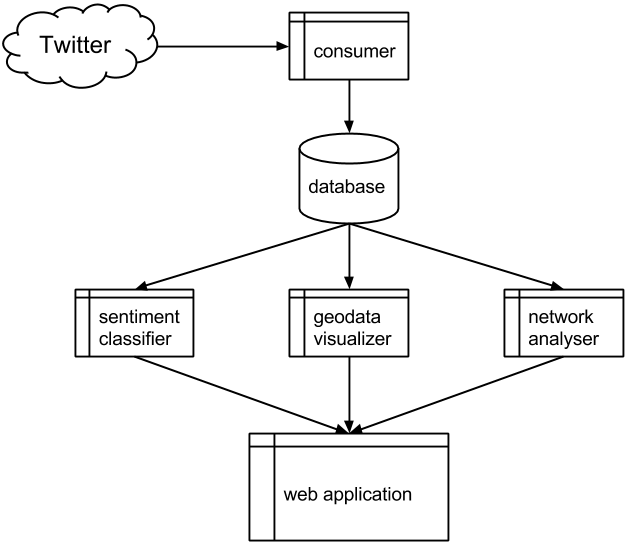
\includegraphics[width=120mm]{img/budowa-systemu.png}
\caption{Gruboziarnisty model systemu}
\label{image:model-systemu}
\end{figure}
- gruboziarnisty schemat systemu

- opis modelu

\subsection{Opis modułów systemu}
[z uwzględnieniem novum]

- twitter listener (słowa kluczowe)

- sentiment classifier (paroubek, dokładnie, dlaczego takie podejście)

- geodata visualizer (google maps, open street maps, cartodb)

- network analyser (gephi, cfinder) - omówić wykorzystanie

- novum: połączenie tych trzech obszarów w jeden

\subsection{Narzędzia użyte do budowy systemu}
- PostgreSQL

- Maven

- Git

- Java (Crawler - Twitter4j, Classifier, Geodata - REST API)

- IntelliJ IDEA

- pgAdmin III

- Play Framework

- Google Charts / JavaScript

- Google Maps, Open Street Maps, CartoDB Maps 


\newpage \section{[Dyskusja wyboru rozwiązania]}
- Twitter -- publiczne wypowiedzi, nastawaiony na komentowanie wydarzeń na żywo,
wspiera geolokalizację

- Paroubek Sentiment Classifier -- krótkie wypowiedzi, świetnie się do nich
nadaje (porównać do innych rozwiązań, dlaczego nie gotowy słownik,
dlaczego nie Naive Bayes), jak zastosowano negację, co ze słowami kluczowymi,
zastosowanie emotikon

- Gephi - otwarty, posiada wiele algorytmów

- CFinder - ułatwia szukanie grup

- Google Charts / Maps - wygodne, dobre API do do wykresów i map

- Open Street Map - otwarty projekt, API do wyciągania informacji o miejscu
na podstawie współrzędnych geograficznych

- moje rozwiązanie jest interesujące ponieważ łączy 
trzy ciekawe obszary w jeden, dotąd nie łączone

\subsection{Ograniczenia, porównania z innymi podobnymi systemami, złożoność}
- nie każdy ma Twittera -- badanie obarczone jest pewnym błędem,
jeśli chciałoby się jego wyniki przypisać całej społeczności

- niewiele osób włącza geolokalizację (domyślnie wyłączona)

- badanie języka jest bardzo trudne (ironia, ukryte żarty, spam, slang, 
szybko zmienijący się zasób słów, okresowa moda na różne określenia, 
skróty, błędy typograficzne, ortograficzne, słowa z obcych języków)


- klasyfikator sentymentu mimo usunięcia słów kluczowych ściśle związany
ze zbiorem uczącym i charakterystyką Twittera - tj. krótkich wypowiedzi 
(do dłuższych recenzji książek, produktów nie spełniłby swojego zadania)
\chapter{Analiza zachowań użytkowników serwisów społecznościowych}

\begin{comment}

\end{comment}
[przykładowe rezultaty działania]

[przykłady działania i ewentualne błędy i dyskusja ograniczeń na podstawie
przykładów]

- opis badanej grupy 
- kibice piłkarscy, anglojęzyczni, 
- 8 mln tweetów, chelsea,
- manchester united, manchester city, arsenal
- głównie Wielka Brytania, USA, Archipelag Malejski, Nigeria, Ghana, Kenia,
Malezja, Singapur, Indonezja, Indie, RPA

\section{Analiza sentymentu}
- bardziej pozytywny, gdy drużyna wygrywa, gdy padają bramki
- spodziewane, intuicyjne wyniki badania sentymentu
\section{Sentyment a geolokalizacja}
- bardziej pozytywny sentyment w mieście drużyny zwycięskiej
- kibice angielscy umiarkowanie zadowoleni
- raczej sentyment w okolicach neutralnego
- kibice amerykańscy, afrykańscy czy malezyjscy cechują się wyższą wartością
sentymentu
\section{Sieci społeczne}
[grupy użytkowników, którzy użytkownicy skupiają na sobie uwagę, jaki niosą sentyment,
jaki generują w ramach swojej grupy]

- najczęściej uwagę (najwyższa wartość miary `authority`, najwyższa wartość
inDegree) skupiają 
oficjalne profile drużyn, które zazwyczaj niosą sentyment neutralny 
-- lekko pozytywny 

- liczba użytkowników biorących udział w wielu wydarzeniach jest
odwrotnie proporcjonalna to liczby tych wydarzeń (im więcej wydarzeń, tym
mniej użytkowników wzięło udział w nich wszystkich)

- największą uwagę skupiają spotkania z największymi rywalami
\chapter{Zakończenie i wnioski}
\section{Podsumowanie}
%%%%%%%%%%%%%%%%%%%%%%%%%%%%%%%%%%%%%%%%%%%%%%%%%%%%%%%%%%%%%%%%%%%%%%%%%%%%%%%%
%%%%  DOPISAĆ O TYM CO UDAŁO SIĘ ZROBIĆ -- DODANO NEGACJE DO ANALIZY SENTYMENTU
%%%%%%%%%%%%%%%%%%%%%%%%%%%%%%%%%%%%%%%%%%%%%%%%%%%%%%%%%%%%%%%%%%%%%%%%%%%%%%%%

W niniejszej pracy próbowano powiązać ze sobą analizę sentymentu i dane
geolokacyjne w celu wzbogacenia analizy użytkowników sieci społecznościowych.
Cel można uznać za osiągnięty.

Analiza sieci społecznych pozwala pokazać w jaki sposób osoby badane łączą się
ze sobą i jaka jest charakterystyka tych połączeń. Pokazuje wielkość
utworzonych grup i ich trwałość.

Zastosowanie analizy sentymentu dostarcza informacje, dzięki którym
możemy odkrywać przyczyny tworzenia się takich a nie innych grup
a także pomaga dowiedzieć się, dlaczego między różnymi grupami występują
konkretne rodzaje relacji. Korzystając z tej dziedziny nauki możemy także
skorelować nastroje społeczne z wydarzeniami na świecie. W niektórych przypadkach
zauważony sentyment może być w miarę przewidywalny -- tak jak w badaniu 
kibiców piłkarskich, gdzie związany jest z wynikiem meczu -- ale w innych
może pozwalać odkrywać niezauważane do tej pory ciągi przyczynowo-skutkowe.

Analiza sieci społecznych może również prowadzić do bogatszych wniosków
poprzez zastosowanie danych związanych z geolokalizacją. Powiązanie informacji
o fizycznym położeniu użytkowników, a także o sentymencie jaki generują
daje dodatkowy obraz pozwalający zrozumieć połączenia między nimi.

Dodatkowo w tej pracy udało się wykorzystać dane pochodzące z serwisu 
społecznościowego -- którym był Twitter.
Jest to bardzo ciekawe medium, które może być szeroko używane do automatycznego
badania nastrojów i sieci społecznych. Pokazano w jaki sposób takie dane
uzyskać, przetworzyć i wykorzystać do podobnych badań. Zaprezentowane zostało podejście,
dzięki któremu badanie dużych grup ludzi można przeprowadzić bez ich wiedzy
i w sposób automatyczny. Dzięki temu uzyskuje się bardziej wiarygodne wyniki.
Użytkownicy nie wiedzą, że są obserwowani i zachowują się w sposób naturalny.


\section{Wpływ pracy na otaczający świat}
Praca ta prezentuje w jaki sposób można połączyć ze sobą analizę sieci społecznych,
analizę sentymentu i analizę geolokalizacji. Udowadnia, że badanie nastrojów
w społeczeństwie można zautomatyzować aplikując komputerowe techniki przetwarzania
dużych zbiorów danych. Pokazuje, że zastosowanie analizy sentymentu i geolokacji
może istotnie wzbogacić analizę dużych grup ludzi.

Zastosowanie automatycznych technik badania dużych sieci społecznych
może uprościć sposoby komunikacji z takimi grupami i odpowiadania na ich potrzeby.
Możemy wyobrazić sobie sytuację, w której rządy, organizacje czy firmy badając
sieci społeczne wraz z analizą i geolokacją błyskawicznie reagują na aktualne
wydarzenia. Przykładem zastosowania takich badań może być prezentowanie
spersonalizowanych reklam. Gdy na przykład dana drużyna przegrywa, jej kibicom
można by wyświetlać po zakończonym meczu inny zestaw reklam niż kibicom drużyny 
przeciwnej. Firmy oferujące swoje usługi czy produkty na całym świecie
mogą szybko reagować na opinie czy błędy zgłaszane przez sfrustrowanych internautów
w serwisach społecznościowych poprawiając swój wizerunek i pokazując dbałość
o klienta. Rządy czy partie polityczne mogą wykorzystać sieci społeczne,
sentyment i geolokacje do odpowiednich zmian, ustaw dotyczących konkretnych grup
społecznych, aby polepszyć wśród nich swoje notowania.

Praca pokazuje, że wykorzystanie mediów internetowych, czy
serwisów społecznościowych może dać wymierne korzyści. Potwierdza, że
świat wirtualny i realny przenikają się. Tak samo reagujemy na różne
wydarzenia niezależnie od tego, czy dzielimy się swoimi opiniami z bliskimi będącymi obok
nas czy z całym światem korzystając z serwisów społecznościowych. Jeśli więc
zarządy firm lub organizacji nie wierzą lub wahają się nad sensem przeprowadzenia
takich badań, to niniejsza praca może być dla nich dowodem, że warto bliżej
przyjrzeć się zaprezentowanym tutaj aspektom. Może być więc punktem wyjścia
do prowadzenia własnych badań na interesujące dany podmiot tematy.



\section{Możliwe kierunki rozwoju}
% plan dalszego rozwoju systemu
% w pływ pracy, zastosowanie wyników teraz i w przyszłości

Zaprezentowana praca jest ukierunkowana na wąską dziedzinę -- bada zachowania
kibiców piłkarskich. W związku z tym, aby rozszerzyć jej zakres konieczne
jest przeprowadzenie kilku działań celem jej rozwoju. Kilka możliwych kierunków to:

\subsubsection{Rozszerzenie o inne języki naturalne}
Zastosowany mechanizm analizy sentymentu jest skupiony jedynie na
języku angielskim. Aby móc badać większe grupy ludzi koniecznym jest opracowanie
techniki badającej również inne języki. Oczywiście w pewnym stopniu można 
wykorzystać podejście zastosowane w tej pracy, należy jednak mieć na uwadze
różnice między budową używanych języków. Zupełnie inne konstrukcje językowe
są w języku angielskim a zupełnie inne na przykład w języku polskim.
Oczywiste jest więc, że nie można w taki sam sposób podejść do badania
wpisów w różnych językach. Rozbudowanie mechanizmu o kolejne języki pozwoliłoby
uzyskać bogatsze wyniki.

\subsubsection{Odkrywanie tematów rozmów}
Ciekawym rozszerzeniem badania sieci społecznych w kontekście przetwarzania
języka naturalnego byłoby opracowanie i zastosowanie metody pozwalającej
odkrywać tematy rozmów użytkowników. W zaprezentowanym podejściu badany jest
jedynie sentyment wpisów, nie ma natomiast informacji na temat tego o czym dokładnie
dyskutują użytkownicy Twittera. Użycie mechanizmu ekstrakcji tematów rozmów
z wpisów z pewnością wzbogaciłoby analizę sieci społecznych.


\subsubsection{Wzbogacenie techniki badania sentymentu}
Badanie wydźwięku wypowiedzi zostało zautomatyzowane. Wykorzystuje do tego celu
wpisy tworzone przez badaną grupę. Interesującym rozszerzeniem techniki badania 
sentymentu mogłoby być zastosowanie ręcznie stworzonego słownika.
Mógłby on nieco skorygować niektóre wyniki analizy wydźwięku wypowiedzi i
polepszyć ich jakość. Dodatkowo pozwoliłoby to na zastosowanie metody analizy sentymentu
w szerszej dziedzinie badań. Aktualna metoda jest w pewien sposób zorientowana
na środowisko piłkarskie i niekoniecznie dawałaby dobre rezultaty w innym
zbiorze danych -- na przykład wpisach politycznych. Skorzystanie ze słownika
i zwięszkenie zakresu badanych wpisów pozwoliłoby szerzej zastosować
opracowaną metodę.

\subsubsection{Bliższe przyjrzenie się grupom}
Dodatkowym kierunkiem rozwoju mogło by być bliższe przyjrzenie się grupom,
które się utworzyły. Można by na przykład skierować swoje badania
na szukanie liderów tych grup, przyczyn ich pojawiania się i sposobów w jaki
oddziałują na resztę grupy w zależności od sentymentu jaki sami generują,
jaki generują dane grupy czy w jakiej lokalizacji geograficznej się znajdują. 






	
\bibliographystyle{plain}
\bibliography{*}
%---------------------------------------------------------------------------
\end{document}
